\documentclass{llncs}

%Packages
\usepackage{amssymb}
\setcounter{tocdepth}{3}
\usepackage{graphicx}
\usepackage{url}

\begin{document}
\mainmatter  

\title{Personalized Nichesourcing: Acquisition of Qualitative Annotations from Niche Communities}
\titlerunning{Personalized Nichesourcing: Acquisition of Qualitative Annotations from Niche Communities}


\author{Chris Dijkshoorn\inst{1}, Mieke Leyssen\inst{2}, Archana Nottamkandath\inst{1}, Jasper Oosterman\inst{3}, Myriam Traub\inst{2}, Lora Aroyo\inst{1}, Wan Fokkink\inst{1}, Geert-Jan Houben\inst{3}}
\authorrunning{Dijkshoorn et. al.}
\tocauthor{Chris Dijkshoorn}
\institute{The Network Institute\\ Department of Computer Science\\ VU University, Amsterdam, the Netherlands\\\email{c.r.dijkshoorn@vu.nl}}
\toctitle{Accurator}


\institute{The Network Institute, VU University, Amsterdam, the Netherlands
\email{\{c.r.dijkshoorn, a.nottamkandath, lora.aroyo, w.j.fokkink\}@vu.nl}
\and Centrum Wiskunde en Informatica, Amsterdam, the Netherlands\\
\email{\{leyssen, traub\}@cwi.nl}
\and Web Information Systems, Delft University of Technology, the Netherlands\\
\email {\{j.e.g.oosterman, g.j.p.m.houben\}@tudelft.nl}
}

\maketitle

\begin{abstract}
% A digital collection that can be accessed online, searched and linked to other collections is an important focus for many cultural heritage institutions. 
Diversity and profundity of the topics in cultural heritage institutions collections make experts from outside the institution indispensable to acquiring qualitative annotations. We define the concept of nichesourcing and present the challenges in the process of obtaining qualitative annotations from persons in these niches. Our assumption is that if this process is personalized, we get better annotations from the experts. We present a framework for nichesourcing, called Accurator, that allows to realize and evaluate strategies and applications for personalized nichesourcing.

\keywords{cultural heritage, nichesourcing, annotation framework, qualitative annotations, user interaction}
\end{abstract}

\section{Introduction}\label{introduction}
Access and retrieval mechanisms for archives and museums rely on a rich description of the collection. Most cultural heritage institutions therefore employ professional experts to describe their collections by manually compiling metadata for each item. For large and diverse collections, this approach can be insufficient to generate precise and comprehensive data. In these cases the knowledge of experts from other domains is indispensable.  Cultural heritage institutions therefore seek to understand whether and how they can exploit the efforts of external users to produce these annotations.

This demo aims at understanding which strategies and techniques lead to high-quality annotations by (crowds of) external experts. The first challenge of the project is to identify the niche of relevant experts and to motivate them to contribute to the annotation of artworks. As a next step, the personalization mechanisms must make sure that the experts are shown items that correspond to their expertise. The quality of the annotations and annotators will be evaluated using trust algorithms. All these aspects must be presented in an appropriate interface.

To evaluate our hypotheses with user studies, we develop a framework designed to support crowd annotation processes, Accurator. The current state of Accurator shows interfaces for two expert niches: castles and flowers. These interfaces are designed for user studies with experts of the respective fields to find out what elements make up a useful interface for them.

\section{Research Challenges}
\label{use_case}

One of the four main challenges of nichesourcing is finding candidate annotators that are able to produce high quality annotations for collection items. 
%Besides topical knowledge, properties like availability, willingness to help and being able to share or transfer knowledge are also important. 
We believe that people participating in a topical community have an active interest in that topic and might be willing to help and share knowledge related it. We refer to these topical communities as \textit{niches} and focus on their manifestation, among others, on the social web. We analyze social data and perform user studies using the Accurator tool to understand what identifies a niche community, what indicates that a person is part of such a community and which properties identify a good candidate to provide qualitative annotations. 

The challenge for recommender strategies in Accurator is twofold: keep the expertise needed to annotate the item in the range of the experts' knowledge and yet diversify the suggestions to get high quality annotations for as many distinct items as possible. 
Our aim is to develop recommender strategies that use content patterns from the Linked Data cloud, resulting in a list of recommendations consisting of diverse items. 
We hypothesize that encountering diverse items to annotate will help keep the expert motivated.

We address issues of determining trust in the expert users and their contributed annotations by modeling the user reputation and tracking their expertise across various topics over time. We believe subjective logic is suitable to model the reputation of users and semantic similarity measures to track and update the users' expertise. Since there is no gold standard for evaluating the annotations, we must rely on a peer reviewing process and other mechanisms such as provenance of the annotation process.
% like tracking provenance of the annotation process such as usage of terms from vocabularies by the user, typing speed etc. We also investigate the different metrics which will help in identifying good behavior of the users. 

% The professional annotation of artworks is a complex process that requires familiarity with the used classification schemes and (art-)historical expert knowledge. Since both will mostly not be available in candidate users for nichesourcing projects,
Since external users are not familiar with professional classification schemes and expert knowledge the institutions target, a fourth main challenge is breaking down the annotation process into facile tasks that can be solved with little effort and without this kind of professional knowledge. %(suggested in \cite{He2013}).
We believe that the interface for such a system has to present the task in a straightforward way while motivating the users to spend the time contributing their knowledge. We investigate which design aspects and underlying mechanisms are responsible for the quality and quantity of tags added by users and how to visualize trust and personalization aspects.



\section{Accurator framework}
\label{architecture}
Our main assumption is that making use of niche sourcing increases the quality of annotations. We believe the we can use specific techniques to identify niches and create user profiles. Based on the user profiles we can recommend relevant tasks to the user and apply trust mechanisms to improve the recommendations. In Figure 1, we show a diagram that represents the workflow of Accurator. 

\begin{figure*}[hbt]
	\centering
	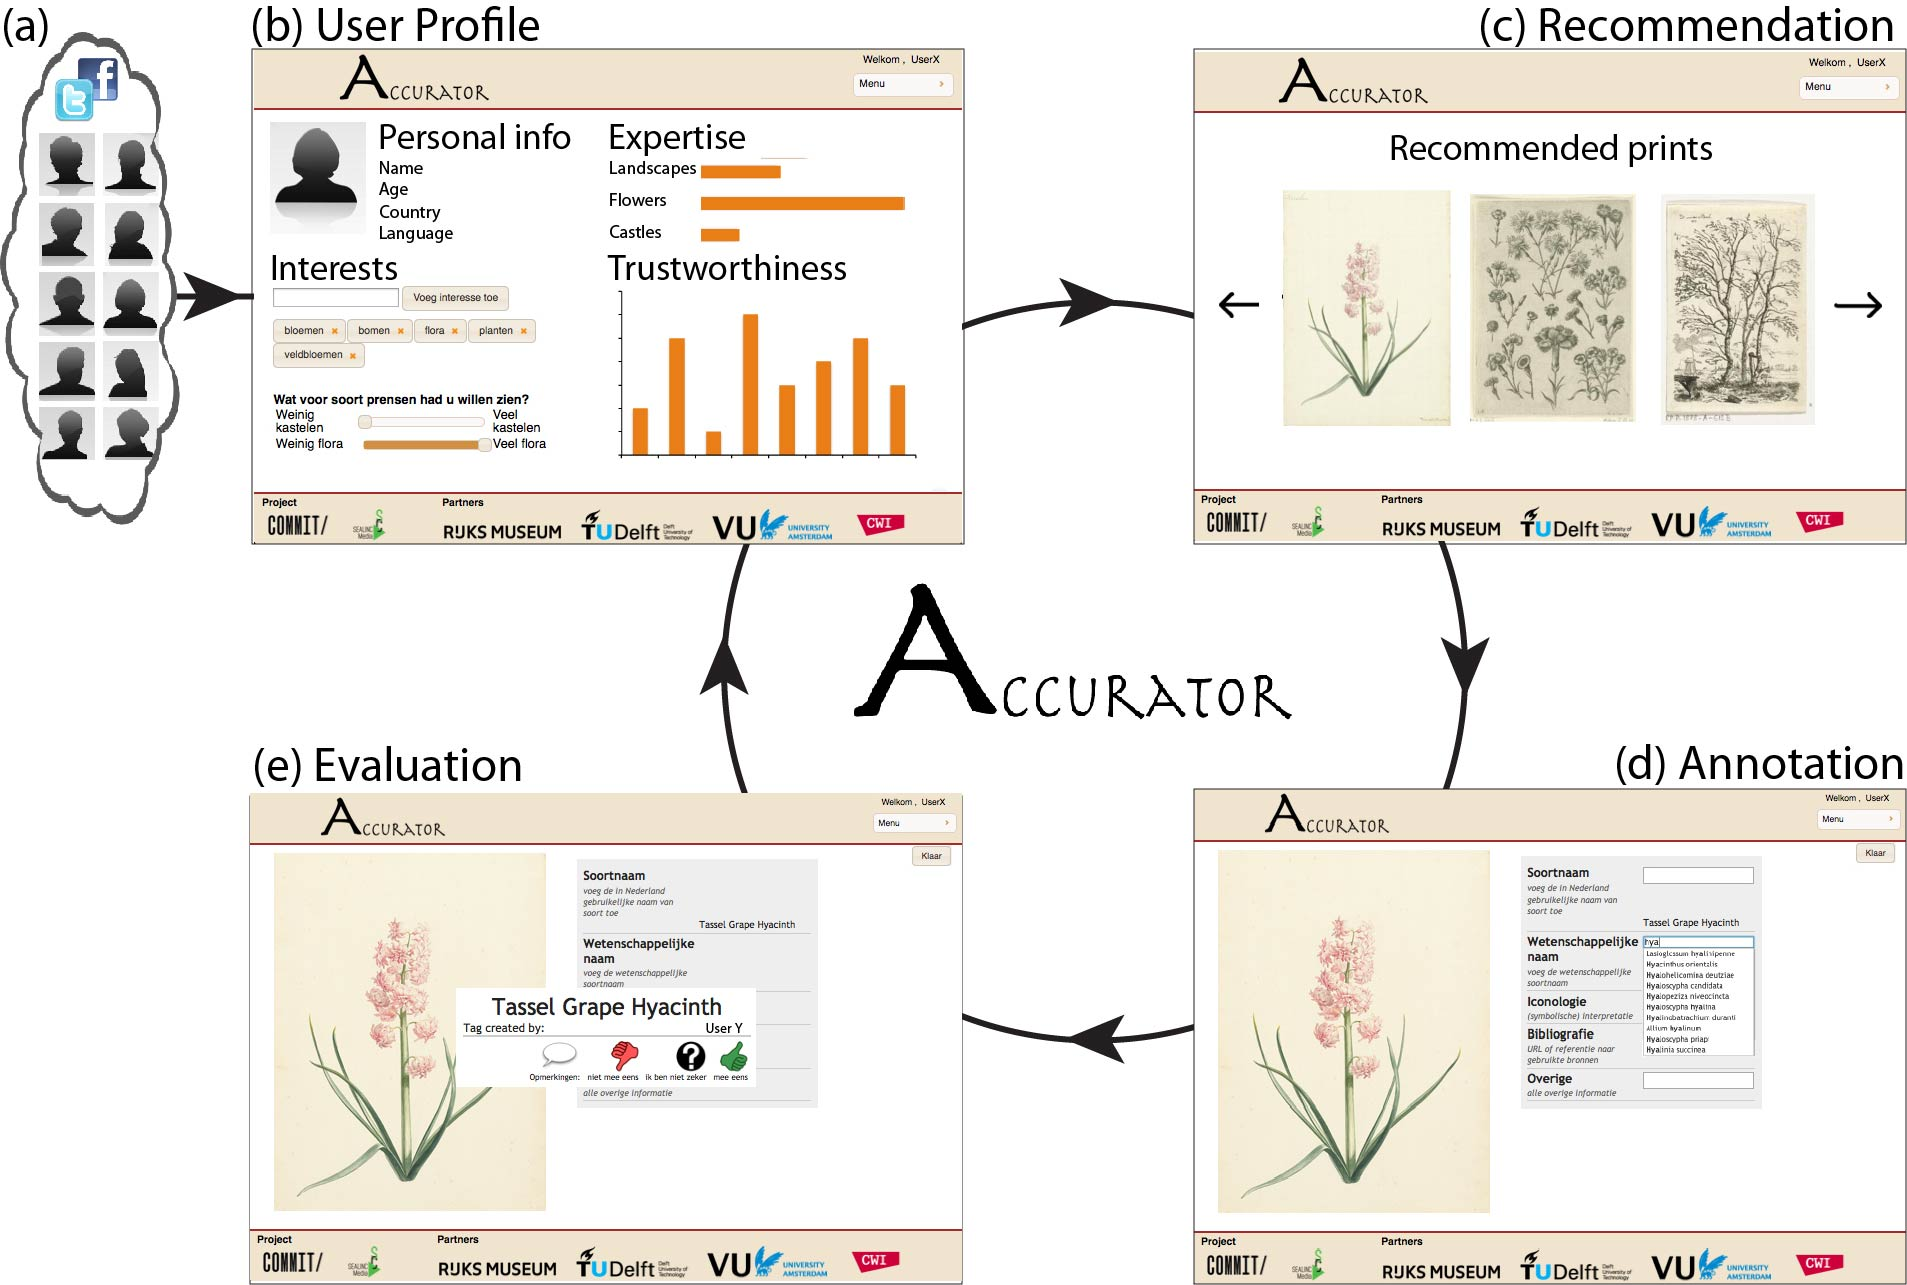
\includegraphics[width=\textwidth]{accurator_diagram.jpg}
  	\caption{Diagram representing the workflow of Accurator}
\end{figure*}

The process starts (see Figure 1a) with searching the social web for user generated content that is relevant for a specific topic. We calculate the relevance of the content creators in respect to the topic and exploit social relations to identify a topical niche. When a person starts using Accurator, a user profile (see Figure 1b) is build based on available data
% and shown to the user. The user can specify additional social web accounts.

Figure 1c shows the recommendation of collection items for a user. The recommendation strategy is based on specific patterns in the data, the user profile and the current annotation quality of an item. Accurator allows to easily change between different strategies to cater for different users.
% and a future task is to automatically adapt the choice of strategy based on that user profile. 
The choice of recommended item will affects the calculated interest of that user.

Figure 1d shows the interface where users add their annotations to an item. The presented fields dependent on the topic and the expertise of the user on that topic. 
%Users with more expertise on that topic are allowed to enter more difficult fields. 
Accurator can also be configured to use a vocabulary for a field to support the user. Figure 1e shows the interface in which users can evaluate the annotations of other users. This task is only available to users who are trustworthy and have a certain level of expertise. The result of a review affects 1) the quality of an annotation, 2) the expertise level of a user and 3) the trustworthiness of another user.

% Another aspect that holds for all interfaces is that they should be intuitive and helpful. Users who encounter difficulties with the interface will not return. 

Accurator is build using Cliopatria to store RDF, GWT for the user interface and GAE for hosting. Accurator is now used for experimentation with data from the Rijksmuseum in the Netherlands and a demo is available at \url{http://rma-accurator.appspot.com}.






\textbf{\\Acknowledgements.}  This publication is supported by the Dutch national program COMMIT. We like to thank the members of the SEALINCMedia worktable and in particular the Rijksmuseum for their support.


\bibliographystyle{splncs03}
\bibliography{bibliography}

\end{document}